% vim: set tw=0:
\documentclass{beamer}
\usepackage{graphicx}
\usepackage{hyperref}
\hypersetup{pdfborder={0 0 0 0}}

% Reasonable themes:
% Antibes Bergen Berkeley Berlin Frankfurt Goettingen Ilmenau Luebeck Malmoe
% Montpellier PaloAlto Rochester Singapore Szeged Warsaw bars boxes
% compatibility default lined plain shadow sidebar split tree
% And these ones include the author's name on every slide:
% Berkeley

% Declare themes.
\mode<presentation>
\usetheme{UWHEP}

% Personal macros.
\newcommand{\email}[1]{{\texttt #1}}
\newcommand{\newframe}[1]{\section{#1}
    \frametitle{\sc{#1}}}
\newcommand{\subframe}[1]{\subsection{#1}
    \frametitle{\sc{#1}}}
\newcommand{\supers}[1]{\ensuremath{^\textrm{#1}}}
\newcommand{\subs}[1]{\ensuremath{_\textrm{#1}}}
\newcommand{\ca}{\ensuremath{\sim}}
\renewcommand{\email}[1]{\href{mailto:#1}{\nolinkurl{#1}}}

% Author information.
\title{T2 Status}
\author[Maier, Mohapatra]{
    Will Maier \and Ajit Mohapatra\\ 
    {\tt wcmaier@hep.wisc.edu}\\
    {\tt ajit@hep.wisc.edu}}
\institute[Wisconsin]{University of Wisconsin - High Energy Physics}
\date{2009.07.21}
\logo{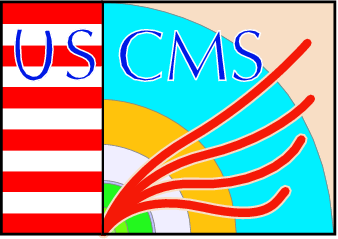
\includegraphics[height=0.6cm]{../../../Graphics/USCMS_logo.png}\hspace{.1cm}
\includegraphics[height=0.75cm]{../../../Graphics/UW_logo.png}}

\begin{document}

\begin{frame}
    \titlepage
\end{frame}

%\section{Overview}
%\begin{frame}
%    \tableofcontents
%\end{frame}

\section{Facilities}
\subsection{Software and Storage}
\begin{frame}
\frametitle{}

\begin{itemize}
	\item Received 56 new nodes for local grid (GLOW; opportunistic access for CMS)
	\item PNFS performance causing SRM transfer hiccups, stuck transfers
	\begin{itemize}
		\item Last month, rolled back upgrade to faster hardware after two failures
		\item Since then, running on old production machine
		\item Stable, but some jobs fail to stage out because PNFS is overloaded
		\item Plan to try upgrade again soon
	\end{itemize}
	\item Two AFS hiccups (no observed effect on SAM and other monitoring)
	\begin{itemize}
		\item Plan to upgrade servers
	\end{itemize}
	\item Cleaned up remaining unlocated files
	\begin{itemize}
		\item Lost during power outages, PNFS failures
	\end{itemize}
	\item Reorganized PoolManager.conf
	\begin{itemize}
		\item PFM, {\tt billingrep} both rely on it to find pools to replicate to
		\item One place to mark pools for drain off (instead of PFM blacklists, etc)
	\end{itemize}
\end{itemize}

\end{frame}

\subsection{Production and Monitoring}
\begin{frame}
\frametitle{}
\begin{itemize}
	\item JobRobot: OK
	\item SAM: OK
	\item RSV: OK
	\item PhEDEx:
	\begin{itemize}
		\item Upgraded to 3\_2\_0 yesterday and both instances are doing Ok
		\item Working with Paul to setup an FTS channel for Wisconsin to enable T2-T2 transfers
		\item Usual MC susbcriptions for local users
	\end{itemize}
	\item MC Production:
	\begin{itemize}
		\item Next round will be pre-production \#2 with 3\_1\_2, which is yet to come
		\item MC production role change for OSG production: see Ken's mail to \email{uscms-t2@fnal.gov}
		\begin{itemize}
			\item Current: {\tt /cms/uscms/Role=cmsprod}
			\item Future: {\tt /cms/Role=production}
			\item Applied for new role this morning; sites can set up mapping in GUMS (and read/write permissions in SE) now
		\end{itemize}
	\end{itemize}
\end{itemize}
\end{frame}

\end{document}
